\documentclass[../main.tex]{subfiles}

\begin{document}
\chapter{Designing and Implementing the Graphics Library} \label{ch:graphics}
    The graphics library is a key component of the system, as it provides the
        functionality for creating images and animations using Haskell.
    The implementation of the graphics library is largely independent of the rest
        of the system.
    It is responsible for generating the necessary data to render images and
        animations, rather than rendering them itself.
    The website described in Chapter~\ref{ch:website} is responsible for rendering
        the images and animations at the correct frame rate, using the data generated
        by the graphics library.

    Throughout this chapter, there are several code snippets taken from the
        implementation of the graphics library.
    In most cases, the implementations are trivial, so have been omitted for
        brevity, and in some cases, verbose type signatures have been replaced with
        ellipses.
    The full implementation of the graphics library can be found in
        Appendix~\ref{app:code}.

    \section{Library Overview}
        There were several sources of inspiration for the graphics library, including
            CodeWorld and P5.js.
        P5.js, as a JavaScript library, is inherently imperative, relying heavily on
            side effects and global state.
        Despite that, it provides a straightforward API, with a nice selection of
            functions, many of which can be adapted to fit the functional paradigm.
        CodeWorld, on the other hand, uses Haskell, so is purely functional, with no
            side effects or global state, relying instead on function composition and
            recursion.
        While CodeWorld's API provides a good example of a functional graphics library,
            it is less straightforward than P5.js.
        The aim for our library is to find a balance between the simplicity of P5.js,
            and the functional design of CodeWorld.

        \subsection{Required Modules}
            The first step in designing the graphics library was to consider what it needed
            to be able to do, from the perspective of a user:
            \begin{itemize}
                \item Represent a two-dimensional space to draw on, i.e. the canvas.
                \item Represent graphical primitives that can be drawn in that space, i.e.
                      shapes.
                \item Apply transformations and colours to these shapes.
                \item Generate the data to allow the website to render the image or animation.
            \end{itemize}

            The graphics library was split into six modules:
            \begin{itemize}
                \item \texttt{Lib} — the main module, which exports the public API for the library.
                      This has one function, \texttt{render}, which takes a \texttt{Canvas} and
                          prints its JSON representation to the standard output.
                      It is the responsibility of the website to render this as an image or
                          animation.
                      This function makes use of Haskell's \texttt{IO} monad, which allows for side
                          effects, such as printing to the standard output.

                      \begin{lstlisting}[language={Haskell}, label={lst:lib}, caption={The 
                        \texttt{render} function.
                        The \texttt{IO ()} return type means that the function has side effects, 
                        specifically printing to the standard output, but no value is returned.}]
render :: Canvas -> IO ()\end{lstlisting}

                \item \texttt{Internal} — an internal module, containing the types and
                      functions used by the library, which are not exposed to the user.
                      This includes the functions to convert each type to their JSON representation.

                \item \texttt{Canvas} — the module for creating and modifying the canvas.

                \item \texttt{Shape} — the module for creating and modifying graphical primitives.

                \item \texttt{Maths} — the module for providing various mathematical functions and
                      types, such as vectors and angles.

                \item \texttt{Color} — the module for providing several representations for colours.
            \end{itemize}

            The following sections will provide an overview of these last four modules.
            This will start with the \texttt{Color} and \texttt{Maths} modules, as they are
                the simplest, and are required by the \texttt{Shape} and \texttt{Canvas}
                modules.

    \section{The \texttt{Color}
        Module}

            \subsection{Common Digital Colour Representations}
                There are several ways to represent colours digitally, each with their own
                advantages and disadvantages.
        Some common representations are hexadecimal, RGB, HSL and HSV.

        \subsubsection{RGB and Hexadecimal}
            The hexadecimal and RGB (red, green, blue) representations are two ways of
                representing the same thing, with the former being more concise, and the latter
                more readable.
            They both represent colours as a combination of red, green and blue, with each
                component being an integer between 0 and 255.
            This is naturally suited to digital displays, which use red, green and blue
                light to create colours.

            RGB uses a tuple of three base ten integers to represent the red, green and
                blue components, respectively.
            This is commonly written as a comma-separated list of integers, enclosed in
                parentheses, prefixed with \texttt{RGB}, e.g. \texttt{RGB(255, 0, 0)} for red.

            Hexadecimal colours combine the red, green and blue components into a single
                base sixteen number.
            This is written as a string, starting with a hash symbol, followed by three
                pairs of hexadecimal digits, representing the red, green and blue components,
                e.g. \texttt{"\#FF0000"} for red.

            These representations can be visualised as a cube, with the x, y and z axes
                representing the red, green and blue components, (see Figure~\ref{fig:rgb}).

            Both RGB and hexadecimal colours can be extended to support an alpha channel,
                allowing for transparency.
            RGB becomes RGBA, with the alpha channel represented as a floating point number
                between 0.0 and 1.0, where 0.0 is transparent, and 1.0 is opaque.
            The alpha channel in hexadecimal colours is represented as another pair of
                hexadecimal digits, with 00 being transparent, and FF being opaque.

            \begin{figure}[H]
                \centering
                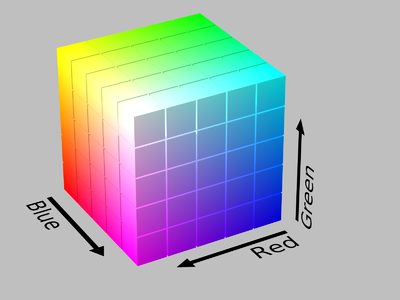
\includegraphics[width=0.35\linewidth]{rgb.png}
                    \caption{The RGB colour space.
                        Image taken from \href{https://en.wikipedia.org/wiki/HSL_and_HSV}{Wikipedia:
                                HSL and HSV}.
                    }
                    \label{fig:rgb}
            \end{figure}

        \subsubsection{HSL and HSV}
            HSL and HSV are almost identical, with HSL representing the colour as a hue,
                saturation and lightness, and HSV (also known as HSB) representing the colour
                as a hue, saturation and value (or brightness).
            These representations are visualised as a cylinder, with the hue, saturation
                and lightness/value components representing the angle, radius and height,
                respectively (see Figure~\ref{fig:hsl}).

            The hue is an angle between 0 and 360 degrees, with 0 and 360 representing red,
                120 representing green, 240 representing blue.
            The saturation is a percentage between 0\% and 100\%, with 0\% being grey, and
                100\% representing a fully saturated colour.
            The lightness/value component is also a percentage between 0\% and 100\%.
            For HSL, 0\% represents black, 100\% represents white, and 50\% represents the
                colour itself.
            For HSV, 0\% represents black, 100\% represents the colour itself, and 50\%
                represents white.

            As with RGB and hexadecimal, HSL and HSV can also be extended to support an
                alpha channel, becoming HSLA and HSVA, with the alpha channel being the same as
                in RGBA.

            \begin{figure}[H]
                \centering
                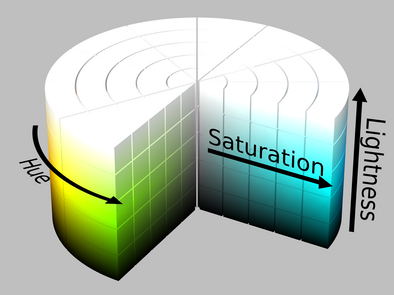
\includegraphics[width=0.35\linewidth]{hsl.png}
                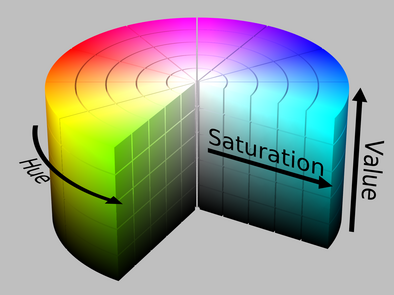
\includegraphics[width=0.35\linewidth]{hsv.png}
                    \caption{The HSL (left) and HSV (right) colour spaces.
                        Images taken from \href{https://en.wikipedia.org/wiki/HSL_and_HSV}{Wikipedia:
                                HSL and HSV}.
                    }
                    \label{fig:hsl}
            \end{figure}

        \subsection{The \texttt{Color}
            Type} For the purposes of this library, it made sense to consider what other
                libraries used for colour representation.
            CodeWorld offers both RGB and HSL, as well as a limited selection of named
                colours.
            P5.js, uses any representation supported by CSS.
            Given that this library is designed to be used in a web browser, it made sense
                to follow P5.js' lead, and support all colour representations that CSS
                supports: hexadecimal, RGB, RGBA, HSL and HSLA, as well as a selection of named
                colours~\citep{cssColours}.

            The \texttt{Color} type has 153 constructors.
            Named colours comprise 148 of these constructors, with the remaining five
                constructors representing the other supported colour representations.

            \begin{lstlisting}[language={Haskell}, label={lst:color}, caption={The \texttt{Color} 
                type definition.
                Named colours have been omitted, but are included in the actual implementation (see 
                Appendix~\ref{app:code}).}]
data Color
    = RGB Int Int Int -- Red, Green, Blue (0-255)
    | RGBA Int Int Int Float -- RGB + Alpha (0.0-1.0)
    | Hex String -- Hexadecimal, # optional, case insensitive
    | HSL Int Int Int -- Hue (0-360), Saturation (0-100), Lightness (0-100)
    | HSLA Int Int Int Float -- HSL + Alpha (0.0-1.0)
    | ... -- Type constructors for named colours omitted\end{lstlisting}

    \section{The \texttt{Maths}
        Module} The majority of the mathematical functions a user would need are
            provided by Haskell's standard library.
        However, there are a few types and functions that are not provided, but are
            useful for a graphics library.

        \subsection{The \texttt{Length}
            Type} The first of these is the \texttt{Length} type, which is used to
                represent lengths, such as the width and height of the canvas, the radius of a
                circle or the side length of a square.
            It is a type alias for \texttt{Float}, providing a level of semantic clarity,
                particularly in the documentation.
            \begin{lstlisting}[language={Haskell}, label={lst:length}, caption={The \texttt{Length} 
                type definition.}]
type Length = Float\end{lstlisting}

        \subsection{Angles}
            There are several units for measuring angles.
            The two most common are degrees and radians.
            Degrees divide a circle into 360 parts.
            This makes it easily divisible by many numbers, but is otherwise arbitrary.
            Radians divide it into $2\pi$ parts, such that one radian is the angle
                subtended at the centre of a circle by an arc equal in length to the radius.
            It made sense to provide users with the ability to work with both of these, and
                functions for converting between them.

            Two more type aliases for \texttt{Float}, \texttt{Degrees} and
                \texttt{Radians}, were defined to provide semantic clarity, as with the
                \texttt{Length} type.
            Functions for converting between degrees and radians were also provided.

            \begin{lstlisting}[language={Haskell}, label={lst:angleFns}, caption={The angle functions.}]  
type Degrees = Float
type Radians = Float                
radians :: Degrees -> Radians
degrees :: Radians -> Degrees\end{lstlisting}

        \subsection{The \texttt{Vector}
            Type} Vectors are a fundamental part of any graphics library, as they can
                represent points, directions, velocities, forces, etc. As this library works
                with just two dimensions, our vectors only need two components, x and y.
            Both P5.js and CodeWorld provide a \texttt{Vector} type, with the latter also
                providing a \texttt{Point} type, which is identical to a \texttt{Vector}.
            For simplicity, we use a single \texttt{Vector} type to represent points,
                directions, and anything else the user may need.
            The \texttt{Vector} type has a single constructor with two type parameters,
                both of type \texttt{Float}.
            Note the use of the \texttt{Float} over \texttt{Length}, as vectors are often
                used to represent several concepts, as mentioned above.
            An alternative to using a custom \texttt{Vector} type would have been to use a
                tuple of \texttt{Float}s, but this would not provide the same level of type
                safety.

            \begin{lstlisting}[language={Haskell}, label={lst:vector}, caption={The \texttt{Vector} 
                type definition.}]
data Vector = Vector Float Float\end{lstlisting}

            \subsubsection{Vector Operations}
                Alongside the \texttt{Vector} type, it is useful to provide a simple set of
                    functions for working with vectors.
                These include addition, subtraction, scalar multiplication, scalar division,
                    dot product, magnitude, argument and normalisation.
                For the first four functions, the \texttt{Vector} type could have been made an
                    instance of the \texttt{Num} type class.
                This would have required us to define all the functions in \texttt{Num}, which
                    is unnecessary, as we only need a subset of them.
                Moreover, there is no defined division or multiplication for vectors, so it
                    would be misleading to make \texttt{Vector} an instance of \texttt{Num}.
                We can instead define the operators \verb|^+^|, \verb|^-^|, \verb|^*^| and
                    \verb|^/^|.
                These names reflect the standard \verb|+|, \verb|-|, \verb|*| and \verb|/|
                    operators, but wrapped by carets (\verb|^|) to indicate that they are for
                    vectors, based on the standard mathematical notation for vectors, which uses a
                    caret above the vector symbol.

                \begin{lstlisting}[language={Haskell}, label={lst:vectorOps}, caption={The vector 
                    operators.}]
-- Vector addition
(^+^) :: Vector -> Vector -> Vector
-- Vector subtraction
(^-^) :: Vector -> Vector -> Vector
-- Scalar multiplication
(^*^) :: Vector -> Float -> Vector
-- Scalar division
(^/^) :: Vector -> Float -> Vector\end{lstlisting}

                The remaining functions are equally simple to define, and make use of several
                    functions from the \texttt{Prelude} module.
                Note that there is no cross product function, as this is only defined for
                    three-dimensional vectors.

                \begin{lstlisting}[language={Haskell}, label={lst:vectorFns}, caption={The remaining 
                    vector functions.}]
-- Calculates the magnitude (length) of a vector
mag :: Vector -> Length
-- Calculates the argument (polar angle) of a vector
arg :: Vector -> Radians
-- Normalises a vector, i.e. returns a vector with the same direction, but a magnitude of 1
norm :: Vector -> Vector
-- Calculates the dot product of two vectors
dot :: Vector -> Vector -> Float\end{lstlisting}

        \subsection{Random Numbers}
            Finally, a set of functions for generating random numbers can be useful for
                creating more interesting animations, allowing for a level of unpredictability.
            As users are not able to access Haskell's \texttt{System} module with the
                online editor, they cannot use the \texttt{System.Random} functions for
                generating random numbers.
            Instead, a simple pseudo-random number generator was implemented using a linear
                congruential generator, which is a simple algorithm for generating
                pseudo-random numbers.
            This algorithm is defined by the recurrence relation $$X_{n+1} = (aX_n + c)
                    \text{ mod } m$$ where $X_0$ is the seed, $a$ is the multiplier, $c$ is the
                increment, and $m$ is the modulus.

            \begin{lstlisting}[language={Haskell}, label={lst:random}, caption={The random number 
                generator which uses a linear congruential generator to generate  an  infinite list
                of pseudo-random numbers, mapped to the range [0, 1].}]
randoms :: Int -> [Double]
randoms seed = map fst (iterate (lcg . snd) (lcg seed))
  where
    lcg :: Int -> (Double, Int)
    lcg seed = (fromIntegral newSeed / fromIntegral (2 ^ 32), newSeed)
      where
        newSeed = (1664525 * seed + 1013904223) `mod` 2 ^ 32\end{lstlisting}

            The values of the multiplier ($a=1664525$), the increment ($c=1013904223$) and
                the modulus ($m=2^{32}$) are taken from Equation~7.1.6, An Even Quicker
                Generator, in Chapter~7.1 of Numerical Recipes~\citep{numericalRecipes}.

            A simple function to generate a seed was also implemented, using the current
                time from the \texttt{Data.Time.Clock.POSIX} module's \texttt{getPOSIXTime}
                function.
            Although the \texttt{getPOSIXTime} function does not come from Haskell's
                \texttt{Prelude} module, it is still safe to use, as it has no side effects,
                and the \texttt{System} module is not exposed to the user.

            \begin{lstlisting}[language={Haskell}, label={lst:seed}, caption={The \texttt{seed} 
                function.}]
seed :: IO Int
seed = do
  time <- getPOSIXTime
  return (floor (time * 1000000))\end{lstlisting}

            The \texttt{seed} function returns an \texttt{IO Int}, as it requires the
                current time to generate the seed, which is not known until runtime.
            The IO monad manages side effects in Haskell in a purely functional manner.

    \section{The \texttt{Shape}
        Module} The \texttt{Shape} module is the most complex, and most important.
        It is responsible for creating and modifying shapes that can be drawn on the
            canvas.
        The module is split into two parts: graphical primitives and transformations.

        \subsection{Graphical Primitives}
            Graphical primitives are the basic building blocks for creating images and
                animations.

            \subsubsection{Examples from P5.js and CodeWorld}
                Once again, it made sense to use a similar set of primitives to those found in
                    P5.js and CodeWorld, as they are simple and easy to use, making them accessible
                    for beginners.
                An initial idea was to more or less translate the P5.js primitives to Haskell.
                This proved to be an inelegant solution, as many functions in P5.js have side
                    effects, which would not work in a purely functional library.
                Instead, it seemed more appropriate to look at the names of these functions,
                    but alter their parameters, and in some cases behaviours, to better suit our
                    library.

                P5.js provides nine primitives: \texttt{point}, \texttt{line},
                    \texttt{triangle}, \texttt{quad}, \texttt{rect}, \texttt{square},
                    \texttt{ellipse}, \texttt{circle} and \texttt{arc}.
                It also provides two functions for creating curves, which it does not describe
                    as primitives: \texttt{bezier} and \texttt{curve}, the former for both
                    quadratic and cubic Bézier curves, and the latter for Catmull-Rom spline
                    curves.
                CodeWorld also provides nine primitives, along with variations to differentiate
                    between certain properties such as filled and outlined shapes, which are
                    omitted here: \texttt{blank}, \texttt{polyline}, \texttt{polygon},
                    \texttt{curve}, \texttt{rectangle}, \texttt{circle}, \texttt{arc},
                    \texttt{sector} and \texttt{lettering}.

            \subsubsection{Our Primitives}
                The primitives provided in this library needed to be simple, easy to use, and
                    cover a wide range of use cases.
                All of our primitives are represented by one \texttt{Shape} type, with eight
                    constructors.
                Each of these, except for \texttt{Empty} and \texttt{Group}, take a parameter
                    of type \texttt{ShapeOptions} to represent the position (\texttt{Vector}),
                    angle (\texttt{Radians}), fill colour (\texttt{Color}), stroke colour
                    (\texttt{Color}) and stroke weight (\texttt{Float}).
                The remaining constructors and their parameters are as follows:
                \begin{itemize}
                    \item \texttt{Empty}, representing the empty shape.
                          This has no type parameters, and drawing it has no effect.
                    \item \texttt{Group}, representing a group of shapes.
                          This has a single type parameter of type \texttt{[Shape]}.
                    \item \texttt{Line}, representing a straight line.
                          This has just one type parameter, of type \texttt{Length}, representing the
                              line's length.
                    \item \texttt{Ellipse}, representing an ellipse.
                          This has two type parameters, both of type \texttt{Length}, representing the
                              ellipse's horizontal and vertical radii.
                    \item \texttt{Rect}, representing a rectangle.
                          This has two type parameters, both of type \texttt{Length}, representing the
                              rectangle's width and height.
                    \item \texttt{Polygon}, representing any polygon.
                          This has one type parameter, of type \texttt{[Vector]}, representing the
                              polygon's vertices.
                    \item \texttt{Curve}, representing both quadratic and cubic Bézier curves.
                          This has one type parameter, of type \texttt{[Vector]}, representing the
                              curve's control points.
                    \item \texttt{Arc}, representing an arc.
                          This has five type parameters.
                          Two of type \texttt{Length}, representing the horizontal and vertical radii of
                              the arc, two of type \texttt{Radians}, representing the start and end angles of
                              the arc, and one of type \texttt{Connection}, representing how the arc closes
                              (either \texttt{Open}, \texttt{Chord} or \texttt{Pie}).
                \end{itemize}

                \begin{lstlisting}[language={Haskell}, label={lst:shape}, caption={The \texttt{Shape} 
                    type definition.}]
data Connection = Open | Chord | Pie
data ShapeOptions = ShapeOptions
    { _position :: Vector
    , _angle :: Radians
    , _fill :: Color
    , _stroke :: Color
    , _strokeWeight :: Float
    }
data Shape
    = Empty
    | Group [Shape]
    | Line
        { _length :: Length
        , _options :: ShapeOptions
        }
    | Ellipse
        { _horizontalAxis :: Length
        , _verticalAxis :: Length
        , _options :: ShapeOptions
        }
    | Rect
        { _width :: Length
        , _height :: Length
        , _options :: ShapeOptions
        }
    | Polygon
        { _points :: [Vector]
        , _options :: ShapeOptions
        }
    | Curve
        { _points :: [Vector]
        , _options :: ShapeOptions
        }
    | Arc
        { _horizontalAxis :: Length
        , _verticalAxis :: Length
        , _startAngle :: Radians
        , _endAngle :: Radians
        , _connect :: Connection
        , _options :: ShapeOptions
        }\end{lstlisting}

                The \texttt{Shape} type is an abstract data type — it is exposed to the user,
                    but its constructors are not.
                The user interacts with the library through the functions in
                    Listing~\ref{lst:shapes}, which construct the required shapes.
                This allows the user to create shapes with default options, and then modify
                    them as needed.
                For every shape, the default options are as follows:
                \begin{itemize}
                    \item The position is the canvas origin, i.e. \texttt{Vector 0 0}.
                    \item The angle is 0 radians.
                    \item The fill colour is \texttt{Transparent}.
                    \item The stroke colour is \texttt{Black}.
                    \item The stroke weight is 1.
                \end{itemize}

                \begin{lstlisting}[language={Haskell}, label={lst:shapes}, caption={The functions to 
                    create shapes.}]
empty :: Shape
line :: Length -> Shape
ellipse :: Length -> Length -> Shape
circle :: Length -> Shape
rect :: Length -> Length -> Shape
square :: Length -> Shape
polygon :: [Vector] -> Shape
regular :: Int -> Length -> Shape
bezier2 :: Vector -> Vector -> Shape
bezier3 :: Vector -> Vector -> Vector -> Shape
arc :: Length -> Length -> Radians -> Radians -> Shape
segment :: Length -> Length -> Radians -> Radians -> Shape
pie :: Length -> Length -> Radians -> Radians -> Shape\end{lstlisting}

                Many of these functions directly correspond to the constructors of the
                    \texttt{Shape} type.
                The \texttt{circle} and \texttt{square} functions are simply special cases of
                    the \texttt{ellipse} and \texttt{rect} functions, respectively.
                The \texttt{regular} function is used to create regular polygons, and takes two
                    arguments: the number of sides, and the radius of the circumcircle.
                The \texttt{bezier2} and \texttt{bezier3} functions are used to create
                    quadratic and cubic Bézier curves, and take two and three control points,
                    respectively.
                They use the \texttt{Curve} constructor, but with a different number of control
                    points.
                The \texttt{arc}, \texttt{segment} and \texttt{pie} functions all use the
                    \texttt{Arc} constructor, but with different values for the \texttt{Connection}
                    parameter; \texttt{Open}, \texttt{Chord} and \texttt{Pie}, respectively.

                The final constructor is the \texttt{Group} constructor, which is used to group
                    shapes together.
                This is useful for creating more complex shapes, as well as for applying
                    transformations to multiple shapes at once.
                To create a group of shapes, the user can use the \verb|&| operator.
                This is a simple infix operator that takes two shapes, and returns a group of
                    those shapes.
                The name of the operator is taken directly from CodeWorld, where it is also
                    used to group shapes together.

                \begin{lstlisting}[language={Haskell}, label={lst:group}, caption={The group (\texttt{\&}) operator.}]
(&) :: Shape -> Shape -> Shape\end{lstlisting}

        \subsection{Transformations}
            There are broadly speaking two categories of transformations to consider:
                colour transformations and geometric transformations.

            \subsubsection{Colour Transformations}
                Colour transformations change the colour of a shape.
                Several colour transformations are commonly used in graphics libraries,
                    including setting the fill colour, setting the outline colour, and setting the
                    outline thickness.
                In P5.js, this is done using the \texttt{fill}, \texttt{stroke} and
                    \texttt{strokeWeight} functions, respectively.
                These alter a global state, so that all subsequent shapes are drawn with the
                    specified properties.
                In CodeWorld, setting the stroke colour is done using the \texttt{colored}
                    function and the regular variant of the shape function (e.g. \texttt{circle}),
                    while setting the fill colour is done using the \texttt{colored} function and
                    the solid variant of the shape function (e.g. \texttt{solidCircle}).
                The stroke weight can be increased by using the thick variant of the shape
                    function (e.g. \texttt{thickCircle}).

                P5.js' approach is more user-friendly, as it allows the user to set the fill,
                    stroke and stroke weight for each shape more easily, but CodeWorld's approach
                    is more functional, as it avoids global state.
                Our design takes the best of both, by retargeting the P5.js functions to
                    transform a given shape, rather than to set a global variable.

                \begin{lstlisting}[language={Haskell}, label={lst:colour}, caption={The colour 
                    transformation functions.}]
-- Sets the fill colour of shape
fill :: Color -> Shape -> Shape
-- Sets the stroke colour of shape
stroke :: Color -> Shape -> Shape
-- Sets the stroke weight of shape
strokeWeight :: Float -> Shape -> Shape
-- Shorthand for fill Transparent
noFill :: Shape -> Shape
-- Shorthand for stroke Transparent
noStroke :: Shape -> Shape\end{lstlisting}

            \subsubsection{Geometric Transformations}
                Several geometric transformations are commonly used in graphics libraries,
                    including translations, rotations and scaling.
                In P5.js, individual shapes do not need to be translated, as the user specifies
                    the position of each shape when creating it.
                Instead, P5.js' \texttt{translate} function moves the canvas' origin, so that
                    all subsequent shapes are drawn relative to the new origin.
                This can be useful but also confusing, particularly for beginners.
                The \texttt{rotate} and \texttt{scale} functions behave similarly, acting on
                    the canvas coordinates rather than individual shapes.
                CodeWorld takes a more intuitive approach, providing functions for translating,
                    rotating and scaling individual shapes.
                This library followed CodeWorld's approach, as it fits better with the
                    functional programming paradigm, and is more intuitive for beginners.

                \begin{lstlisting}[language={Haskell}, label={lst:geometric}, caption={The geometric 
                    transformation functions.}]
-- Moves a shape to a new position
translate :: Vector -> Shape -> Shape
-- Rotates a shape by a given angle
rotate :: Radians -> Shape -> Shape
-- Scales a shape by a given factor
scale :: Float -> Shape -> Shape
-- Shorthand for translate (Vector x 0)
translateX :: Length -> Shape -> Shape
-- Shorthand for translate (Vector 0 y)
translateY :: Length -> Shape -> Shape\end{lstlisting}

            \subsubsection{Applying Transformations}
                Transformations can be applied to a shape by directly calling the appropriate
                    function.

                \begin{lstlisting}[language={Haskell}]
translate (Vector 10 10) (rotate (radians 45) (scale 2 (rect 100 100)))\end{lstlisting}

                This can be cumbersome, particularly when applying multiple transformations to
                    a shape.
                Another approach would be to compose the functions, then apply the resulting
                    function to the shape.

                \begin{lstlisting}[language={Haskell}]
transformation = translate (Vector 10 10)
               . rotate (radians 45)
               . scale 2
transformation(rect 100 100)\end{lstlisting}

                This makes that specific combination of transformations reusable, and more
                    readable.
                However, as the order of the transformations is reversed, this could still be
                    confusing for beginners.
                To solve this, an operator was implemented specifically for applying
                    transformations to shapes.

                \begin{lstlisting}[language={Haskell}, label={lst:transform}, caption={The 
                    transformation application (\texttt{>>>}) operator.}]
(>>>) :: Shape -> (Shape -> Shape) -> Shape\end{lstlisting}

                Now, the user can apply transformations to shapes in a readable and intuitive
                    fashion.

                \begin{lstlisting}[language={Haskell}]
rect 100 100 >>> scale 2
             >>> rotate (radians 45)
             >>> translate (Vector 10 10)\end{lstlisting}

    \section{The \texttt{Canvas}
        Module} This is responsible for creating and modifying the canvas.
        The \texttt{Canvas} type has five type parameters:
        \begin{itemize}
            \item Two \texttt{Length}s to represent the width and height.
            \item An \texttt{Int} to represent the frame rate at which to render the animation.
            \item A \texttt{Color} to represent the background colour to apply to each frame.
                  There is an argument for omitting this, requiring users to draw a rectangle
                      filling the whole canvas, and applying the background colour there.
                  However, as most animations are likely to use the same background colour for
                      each frame, this provides a more elegant solution.
            \item A \texttt{[Shape]} to represent the frames of the animation.
        \end{itemize}

        \begin{lstlisting}[language={Haskell}, label={lst:canvas}, caption={The \texttt{Canvas} type 
            definition.}]
data Canvas = Canvas
    { _width :: Length
    , _height :: Length
    , _fps :: Int
    , _backgroundColor :: Color
    , _frames :: [Shape]
    }\end{lstlisting}

        Once the \texttt{Canvas} type was defined, we needed an interface for users to
            interact with it, starting with a function to create a canvas.
        One option was to take all the canvas parameters as arguments.
        However, this would require the user to write out each parameter in every
            program they write, even if these values are not important to them.
        To provide a more user-friendly interface, the function provides default values
            for certain parameters, requiring the user to only specify the width and
            height.
        Specifically, the default values for the frame rate and background colour are
            24 and \texttt{Transparent}, respectively, while the default value for the
            frames is an empty list.
        To modify the frame rate and background colour, the \texttt{fps} and
            \texttt{background} functions were provided.

        \begin{lstlisting}[language={Haskell}, label={lst:fps}, caption={The \texttt{createCanvas}, \texttt{fps} and 
            \texttt{backgrounds} functions.}]
createCanvas :: Length -> Length -> Canvas
fps :: Int -> Canvas -> Canvas
background :: Color -> Canvas -> Canvas\end{lstlisting}

        To allow the user to draw shapes on the canvas, we needed a way to append
            shapes to the list of frames.
        This was handled by two operators, \texttt{(<<<)}, which adds a single
            \texttt{Shape}, and \texttt{(<<<:)}, which appends a list of \texttt{Shape}s.
        The \texttt{(<<<:)} operator was not strictly necessary, as users could instead
            use \texttt{foldl (<<<) canvas shapes}, but it provided a more elegant
            solution.
        Using \texttt{foldl} with \texttt{(<<<)} would not allow the user to take
            advantage of Haskell's lazy evaluation, as the list of shapes would be fully
            evaluated due to the tail-recursive nature of \texttt{foldl}.

        \begin{lstlisting}[language={Haskell}, label={lst:<<<}, caption={The operators to append a 
            frame to the canvas.}]
(<<<) :: Canvas -> Shape -> Canvas
(<<<:) :: Canvas -> [Shape] -> Canvas\end{lstlisting}

        A final function was defined within the \texttt{Canvas} module, to translate
            shapes to the centre of the canvas.
        It was defined in this module because it requires the canvas as an argument, as
            well as the shape.
        Defining it in the \texttt{Shape} module would require importing the
            \texttt{Canvas} module, which would create a circular dependency.

        The implementation of this translation was dependent on the shape's origin.
        For shapes whose origin is at their centre, such as circles and ellipses,
            centring the shape was as simple as translating it by half the width and height
            of the canvas.
        For shapes whose origin is at their top-left corner, such as rectangles and
            polygons, centring the shape was more complex.
        It required translating the shape by half the width and height of the canvas,
            then translating it back by half the width and height of the shape.
        These shapes also needed to be translated to account for their rotation.

        \begin{lstlisting}[language={Haskell}, label={lst:centre}, caption={The \texttt{center} 
            function.}]
center :: Canvas -> Shape -> Shape\end{lstlisting}

\end{document}
